\documentclass[conference]{IEEEtran}
\IEEEoverridecommandlockouts

\usepackage{hyperref}
\usepackage{amsmath,amssymb,amsfonts,nccmath}
\usepackage{algorithmic}
\usepackage[table,xcdraw]{xcolor}
\usepackage{graphicx}
\usepackage{textcomp}
\usepackage{xcolor}
\usepackage[utf8]{inputenc}
\usepackage{multirow}
\usepackage{textcomp}
\usepackage{longtable}
\usepackage{latexsym}
\usepackage{url}
\usepackage[switch]{lineno}
\usepackage[labelformat=parens]{subfig}
\usepackage[inline]{enumitem}
\usepackage{lipsum}
\usepackage{footnote}
\usepackage{comment}
\usepackage{caption}

\makeatletter
\newcommand*{\rom}[1]{\expandafter\@slowromancap\romannumeral #1@}
\makeatother

\DeclareRobustCommand*{\IEEEauthorrefmark}[1]{%
  \raisebox{0pt}[0pt][0pt]{\textsuperscript{\footnotesize #1}}%
}

\def\BibTeX{{\rm B\kern-.05em{\sc i\kern-.025em b}\kern-.08em
    T\kern-.1667em\lower.7ex\hbox{E}\kern-.125emX}}
\begin{document}

\title{BLG 527E Machine Learning  \\ Project Report
{\footnotesize \textsuperscript{}}
\thanks{}}

\author{
    \IEEEauthorblockN{
        First Author
        \IEEEauthorrefmark{1},
        Second Author
        \IEEEauthorrefmark{1}}
\IEEEauthorblockA{\IEEEauthorrefmark{1} Istanbul Technical University, Department of Computer Engineering \\ İstanbul, Turkey \\
Email: \{first, second\}@itu.edu.tr}
}

\maketitle

\begin{abstract}
% Briefly describe the work in this paper

\end{abstract}

\begin{IEEEkeywords}
%You may add keywords
citation networks, clustering, ...

\end{IEEEkeywords}

\section{Introduction} \label{sec:intro}

% Describe the problem (Clustering of Papers by subject)



% Why do we cluster papers? Why is this important? What uses might it have?




%Share any difficulties encountered/may be involved in solving this problem.




%Briefly describe the clustering model you propose.


\section{Literature Review} \label{sec:lite}

%Find 5 research studies applying clustering for similar topics, published within the last 5 years by one of the publishers of ACM, Springer, IEEE, Elsevier.


% https://scholar.google.com/
%Give an overview of the methods applied in each paper study and their contributions to the literature.
%Evaluate each paper in terms of similarity/difference with our study.

\begin{enumerate}
%Complete the following for each paper, as requested at the beginning of this section. Add and reference the papers to the 'bibliography.bib' file.

    %First Paper:
    \item 
    
    %Second Paper
    \item
    
    %Third Paper
    \item
    
    %Fourth Paper
    \item
    
    %Fifth Paper
    \item

\end{enumerate}


\section{Methodology} \label{sec:meth}


\subsection{Pre-trained Text-to-Vec Models}

%You are expected to explain the 3 different text-to-vec models you used in the coding phase separately below.


A summary of all Pre-trained Text-to-Vec Models is as in Figure \ref{fig_pretrained_models}.


\begin{enumerate}
    %Explain the working logic of the Pre-trained Text-to-Vec Model in your own words.
    \item 
    
    
    %Explain the working logic of the Pre-trained Text-to-Vec Model in your own words.
    \item 
    
    
    %Explain the working logic of the Pre-trained Text-to-Vec Model in your own words.
    \item 
    
    
\end{enumerate}

\begin{figure*}
\centering
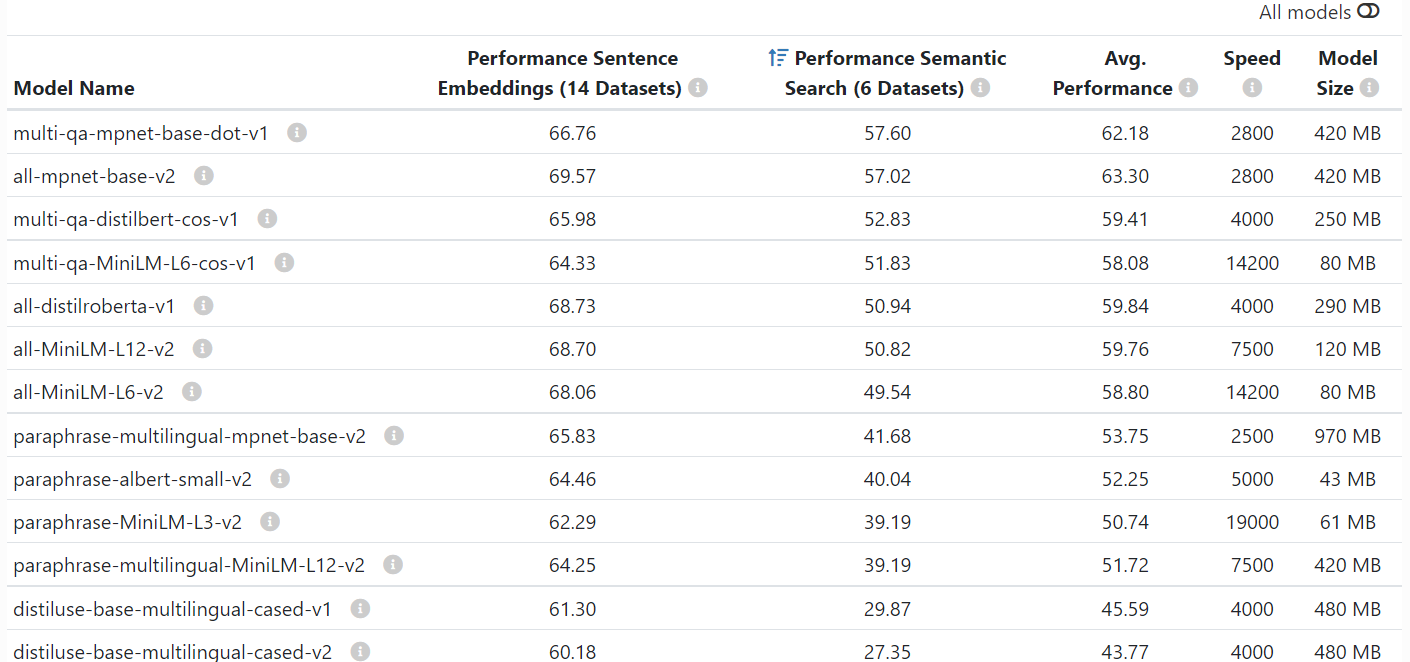
\includegraphics[width=160mm]{pretrained_models.png}
\caption{Pre-trained text-to-vec Models \cite{ref1}}
\label{fig_pretrained_models}
\end{figure*}
\vspace{3pt}



\begin{figure*}
\centering
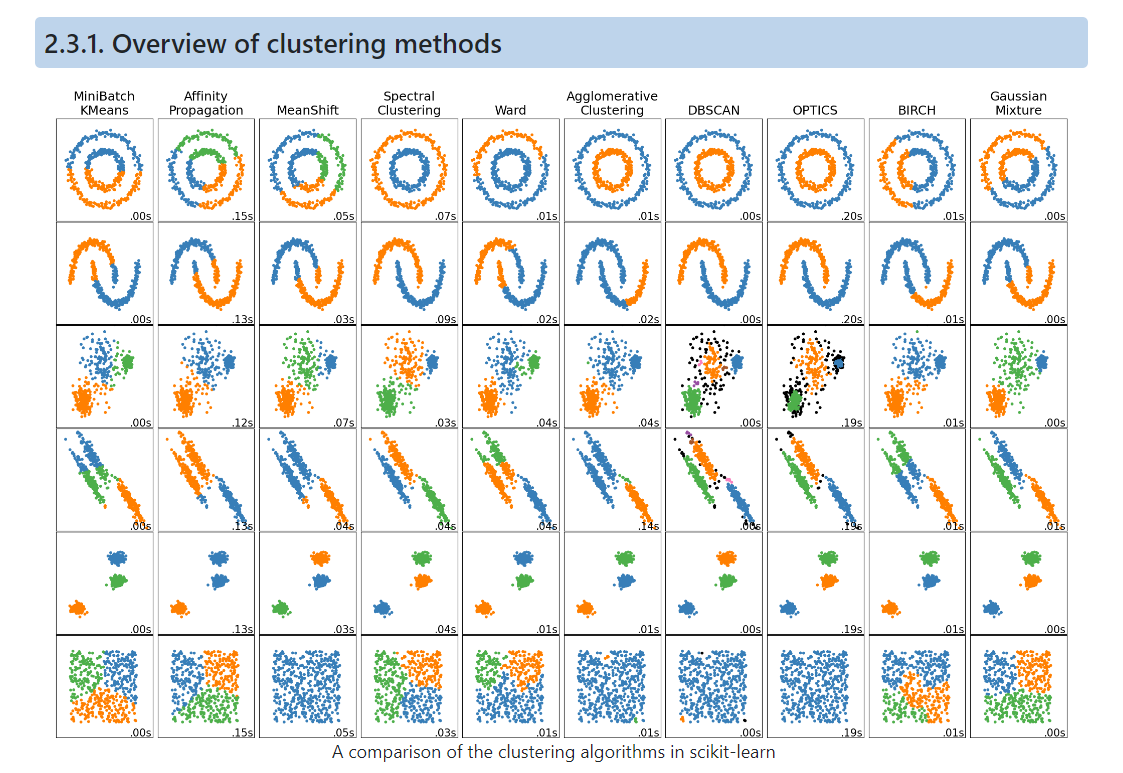
\includegraphics[width=160mm]{clustering_methods.png}
\caption{Clustering Methods \cite{pedregosa2011scikit}}
\label{fig_clustering_methods}
\end{figure*}
\vspace{3pt}


\subsection{Clustering Methods}

%Explain the working logic of the method in your own words by also considering the basic hyperparameters of the method.
\subsubsection{K-means}






%Explain the working logic of the method in your own words by also considering the basic hyperparameters of the method.
\subsubsection{Spectral Clustering}






%Explain the working logic of the method in your own words by also considering the basic hyperparameters of the method.
\subsubsection{Density-Based Spatial Clustering of Applications with Noise (DBSCAN)}






%Explain the working logic of the method in your own words by also considering the basic hyperparameters of the method.
\subsubsection{Gaussian Mixture}





\section{Data Preparation \& Experimental Results} \label{sec:eval}

% Explain how you created the dataset. The number of samples, feature set,...




% Training - Test Datasets Proportions? And the number of samples in each dataset.




%Explain the performance metrics you have chosen, including their working logic and the values they can take, what score they produce in the best case, etc.
% https://scikit-learn.org/stable/modules/clustering.html#clustering-performance-evaluation
\subsection{Clustering Performance Evaluation Metrics}
\begin{itemize}
    % First Performance Metric:
    \item 

    %Second Performance Metric:
    \item 
\end{itemize}

\subsection{Experiments \& Results}


%Obtained Results with this method
%Values obtained with performance metrics, visualizations
\subsubsection{K-means}


%What values have you tried for the hyperparameters of this method?
% For ex. for K-means: k: [2, 3, 4]
\textbf{Hyperparameter Space}




%Obtained Results with this method
%Values obtained with performance metrics, visualizations
\subsubsection{Spectral Clustering}


%What values have you tried for the hyperparameters of this method?
\textbf{Hyperparameter Space}




%Obtained Results with this method
%Values obtained with performance metrics, visualizations
\subsubsection{Density-Based Spatial Clustering of Applications with Noise (DBSCAN)}


%What values have you tried for the hyperparameters of this method?
\textbf{Hyperparameter Space}



%Obtained Results with this method
%Values obtained with performance metrics, visualizations
\subsubsection{Gaussian Mixture}


%What values have you tried for the hyperparameters of this method?
\textbf{Hyperparameter Space}


\section{Proposed Method in this Study}
%Which method stands out as a result of the experiments? 


%What do you think might be the reason for this method to come to the fore?


\section{Clustering Analysis}
%Share your findings and results you obtained for 'Clustering Analysis'.
%1. How many clusters did the model you propose create?
%2. What is the number of papers in each cluster?
%3. What is the unique number of authors in each cluster?
%4. What are the top 3 most frequently used words (the words that describe the cluster) in each cluster?




\section{Clustering of Authors}
%Share your findings and results you obtained for 'Clustering of Authors'.


\section{Future Works}
%If you wanted to improve this work, what could be done? Please share your ideas.
%Fill in below.


\section{Google Drive Link}
%If you have done your work via Google Colab, share the link.

Google Drive Link: 


\bibliographystyle{IEEEtran}
\bibliography{bibliography.bib}
\end{document}



